% Provenance (never printed): see sources/outline_sources.md (Year 3: refraction and
% reflection seismic methods; CMP acquisition, NMO, stacking, Dix; migration in
% principle; seismic stratigraphy). Brief: sources/book5/BRIEFS.md, ch. 2. Curves from
% figdata/bachelor-3/seismic_model.py, refraction_dip.py, synthetic_seismogram.py,
% cmp_nmo.py (the Varden column, region.py); exercise and problem values in the
% Book 5 scratch calculator calc/ch02.py.
\chapter{Exploratieseismologie}\label{ch:b3:exploration-seismology}

Een opnameschip vaart langzaam langs een rechte lijn op zee en sleept een reeks
luchtkanonnen op enkele meters onder het oppervlak en, daarachter, kabels van
meerdere kilometers lang, bezaaid met hydrofoons. In één onderzoek dat aan de
toezichthouder is beschreven, bevatte de reeks \num{5240} kubieke inch perslucht, afgevuurd elke
\qty{8}{s} vanaf \qty{12}{m} onder het oppervlak, en de smalazimut-streamers
achter dergelijke schepen registreren offsets van 8 tot \qty{10}{km}.
% ledger: noaa5:wg-survey
Elk schot stuurt een geluidspuls de zeebodem in, en elk gesteentegrensvlak
eronder geeft een zwakke echo terug. Weken later, na de verwerking, bladert een geoloog
door een doorsnede waarin begraven rivierlopen, gekantelde breukblokken en
de onlappende opvulling van een oud bekken verschijnen alsof de grond open is gesneden.
De seismologie op aardschaal uit het vorige hoofdstuk gebruikte de golven van
aardbevingen; de exploratieseismologie maakt er zelf, met bronnen waarvan tijd en
plaats exact bekend zijn, en registreert ze op duizenden kanalen. Dit
hoofdstuk volgt de echo's van het schot tot de doorsnede: refractieonderzoeken,
de reflectie van een \omterm{def:b3:exploration-seismology:wavelet}{seismische wavelet} door een gelaagde kolom, de methode met \omterm{def:b3:exploration-seismology:cmp}{gemeenschappelijk middelpunt}
die herhaalde echo's omzet in snelheden en een helder beeld, migratie, die
de reflectoren weer op hun plaats zet, en het lezen van de doorsnede als
stratigrafie.

\begin{recall}
Op een grens tussen twee media met akoestische impedanties $Z_1 = \rho_1v_1$ en
$Z_2 = \rho_2v_2$ wordt een vlakke golf bij loodrechte inval gereflecteerd met de
amplitudecoëfficiënt $R = (Z_2 - Z_1)/(Z_2 + Z_1)$ (de natuurkundeboeken, Boek~4,
over golven op grensvlakken). De kopgolf, de intercepttijd en de
kruisingsafstand van een refractieprofiel over vlakke lagen zijn behandeld in
Boek~3, in het hoofdstuk over de gelaagde Aarde; boorstaten in Boek~2
(leerjaar~11). De convolutie $(f*g)(t) = \int f(\tau)g(t - \tau)\,\mathrm d\tau$
en de Fouriertransformatie komen uit de wiskundeboeken. De \omterm{def:b3:seismology-imaging:ray-parameter}{straalparameter} en het
lineair \omterm{def:b3:seismology-imaging:inverse}{invers probleem} zijn die van \cref{ch:b3:seismology-imaging}.
\end{recall}

\section{Refractieonderzoeken}

\begin{definition}[Seismische refractie- en reflectieonderzoeken]\label{def:b3:exploration-seismology:surveys}
Een \emph{seismisch refractieonderzoek}\index{seismisch refractieonderzoek} registreert, langs
een lijn van ontvangers, de eerste aankomsten van een gecontroleerde bron, en gebruikt de
kopgolven die langs de bovenkant van snellere lagen lopen om hun snelheden en
diepten te bepalen. Een \emph{seismisch reflectieonderzoek}\index{seismisch reflectieonderzoek}
registreert de volledige golftrein, bij offsets die meestal kleiner zijn dan de diepten van
belang, en gebruikt de golven die bij bijna loodrechte inval door de
grensvlakken worden gereflecteerd om de lagenbouw in beeld te brengen.
\end{definition}

Boven vlakke lagen komt een kopgolf aan op $t = x/v_2 + t_i$, een rechte lijn
waarvan de helling de snelheid $v_2$ van de refractor geeft en waarvan het snijpunt $t_i$
geeft de diepte ervan. Een hellende refractor kantelt de lijn: de kopgolf van een schot
naar beneden langs de helling komt steeds later aan, naarmate de refractor dieper ligt, en lijkt traag;
tegen de helling in geschoten lijkt hij snel. Door in beide richtingen langs dezelfde lijn te schieten, een omgekeerd
profiel, scheidt de snelheid van de helling.

\begin{theorem}[Refractie op een hellend grensvlak]\label{thm:b3:exploration-seismology:dipping}
Een laag met snelheid $v_1$ ligt op een vlakke refractor met snelheid $v_2 > v_1$ die
onder de hoek $\theta$ langs het profiel helt; $i_c = \arcsin(v_1/v_2)$, en $h$ is de
loodrechte diepte van de refractor onder het schot. Voorbij de kritieke
afstand komt de kopgolf aan bij
\begin{align*}
  t &= \frac{x\sin(i_c + \theta)}{v_1} + \frac{2h\cos i_c}{v_1}
  &&\text{schietend in de hellingrichting},\\
  t &= \frac{x\sin(i_c - \theta)}{v_1} + \frac{2h\cos i_c}{v_1}
  &&\text{schietend tegen de helling in}.
\end{align*}
De schijnbare snelheden $v_d = v_1/\sin(i_c + \theta)$ en
$v_u = v_1/\sin(i_c - \theta)$ van een omgekeerd profiel geven
\[
  i_c = \tfrac12\left[\arcsin\frac{v_1}{v_d} + \arcsin\frac{v_1}{v_u}\right],\qquad
  \theta = \tfrac12\left[\arcsin\frac{v_1}{v_d} - \arcsin\frac{v_1}{v_u}\right],
  \qquad v_2 = \frac{v_1}{\sin i_c} .
\]
\end{theorem}

\begin{proof}
Draai het assenstelsel zodat de refractor horizontaal ligt; het oppervlak helt dan onder
$\theta$. Bij schieten in de hellingrichting is de loodrechte diepte onder een ontvanger op
afstand $x$ gelijk aan $h + x\sin\theta$; de projectie daarvan op de refractor
is $x\cos\theta$. Het pad van de kopgolf gaat onder de kritieke hoek $i_c$ naar de
normaal, langs de refractor met $v_2$, en weer omhoog onder $i_c$. Haar tijd is
\[
  t = \frac{h}{v_1\cos i_c} + \frac{x\cos\theta - h\tan i_c - (h + x\sin\theta)\tan i_c}{v_2}
  + \frac{h + x\sin\theta}{v_1\cos i_c}.
\]
Met $1/v_2 = \sin i_c/v_1$ en $1/\cos i_c - \sin i_c\tan i_c = \cos i_c$,
de termen in $h$ geven $2h\cos i_c/v_1$ en die in $x$
geven $x(\sin i_c\cos\theta + \cos i_c\sin\theta)/v_1 = x\sin(i_c + \theta)/v_1$.
Tegen de helling in verandert $\theta$ van teken. De laatste formules inverteren de twee schijnbare
snelheden.
\end{proof}

De twee takken van een omgekeerd profiel moeten dezelfde tijd tussen de twee
schotpunten geven, ongeacht welk uiteinde vuurde: de \emph{reciproke tijd}, een controle op het
picken. Twee situaties maken de methode onbruikbaar. Een laag die trager is dan de laag erboven
(een snelheidsinversie) levert geen kopgolf op en is onzichtbaar: haar gesteenten worden
meegeteld in de laag erboven, en elke diepte eronder wordt overschat. Een laag
die sneller is dan de laag erboven maar te dun is, kan misschien nooit een eerste aankomst opleveren, omdat
de kopgolf van de diepere, snellere laag haar inhaalt: een verborgen laag. Een
reflectieonderzoek ziet beide.

\begin{omfigure}
\begin{tikzpicture}
\begin{axis}[omrecord, width=0.82\linewidth, height=0.46\linewidth,
  xmin=0, xmax=1200, ymin=0, ymax=660,
  xlabel={positie langs de spreiding, vanaf schot W (\unit{m})},
  ylabel={tijd (\unit{ms})}, legend pos=north west, legend cell align=left,
  legend style={font=\scriptsize}]
\addplot[gray, thick, densely dashed] table[x=x, y=tdir] {figdata/out/bachelor-3-refraction_dip-west.dat};
\addlegendentry{directe golven ($v_1$)}
\addplot[blue!70!black, thick] table[x=x, y=thead] {figdata/out/bachelor-3-refraction_dip-west.dat};
\addlegendentry{kopgolf vanuit W, schietend tegen de helling in}
\addplot[red!70!black, thick] table[x expr=1200-\thisrow{x}, y=thead] {figdata/out/bachelor-3-refraction_dip-east.dat};
\addlegendentry{kopgolf vanuit O, schietend in de hellingrichting}
\addplot[gray, thick, densely dashed, forget plot] table[x expr=1200-\thisrow{x}, y=tdir] {figdata/out/bachelor-3-refraction_dip-east.dat};
\addplot[only marks, mark=*, mark size=1.5pt] coordinates {(1200,486.13) (0,486.13)};
\node[font=\scriptsize, anchor=south east] at (axis cs:1190,530) {reciproke tijd};
\end{axis}
\end{tikzpicture}

\par\smallskip{\small Een omgekeerd refractieprofiel op de westelijke flank van de
Varden-antiklinaal (berekend; probleem, deel I). Het refractorvlak, de top van de
kalksteen, stijgt van W naar O onder een hoek van \ang{10.8} onder een spreiding van \qty{1200}{m}; de
krijt- en schalielagen daarboven zijn samengevoegd tot één laag van \qty{2.40}{km.s^{-1}}. De
kopgolf die van W uit omhoog in de helling schiet lijkt snel (\qty{6.57}{km.s^{-1}}), die van O uit
omlaag in de helling langzaam (\qty{3.52}{km.s^{-1}}); beide hebben \qty{486.1}{ms} nodig om de
hele spreiding te doorlopen. De kopgolven halen de directe golven pas dicht bij het verste
uiteinde in: het refractorvlak ligt diep voor zo'n korte spreiding.}
\label{fig:b3:exploration-seismology:refraction}
\end{omfigure}

\section{Reflectie bij normale inval}

\begin{definition}[Seismische wavelet, Ricker-wavelet]\label{def:b3:exploration-seismology:wavelet}
Een \emph{seismische wavelet}\index{seismische wavelet} is de korte puls, enkele tientallen
milliseconden lang, die een bron en het registratiesysteem door de bodem sturen; elke
reflector stuurt een geschaalde kopie ervan terug. De \emph{Ricker-wavelet}\index{Ricker-wavelet} met
piekfrequentie $f$ is de nulfasepuls
\[
  w(t) = \left(1 - 2\pi^2f^2t^2\right)e^{-\pi^2f^2t^2},
\]
de tweede afgeleide van een Gausskromme, op teken en schaal na: een centrale piek en
twee zijlobben, met nulgemiddelde en een amplitudespectrum dat piekt bij $f$.
\end{definition}

\begin{definition}[Reflectiviteitsreeks]\label{def:b3:exploration-seismology:synthetic}
De \emph{reflectiviteitsreeks}\index{reflectiviteitsreeks} van een gelaagde kolom is
de reeks normale-invalsreflectiecoëfficiënten $r_k$ van haar grensvlakken, geplaatst op
hun heen-en-terugtijden $\tau_k = \sum_{i \le k} 2h_i/v_i$:
$r(t) = \sum_k r_k\,\delta(t - \tau_k)$.
\end{definition}

\begin{proposition}[Het convolutiemodel]\label{prop:b3:exploration-seismology:synthetic}
Als alleen primaire reflecties worden meegenomen (geen meervoudige), bij normale inval,
zonder transmissieverlies, demping of uitwaaiering, en als de wavelet $w$ niet
verandert met de diepte, dan is het opgenomen spoor de convolutie van de wavelet met de
\omterm{def:b3:exploration-seismology:synthetic}{reflectiviteitsreeks}:
\[
  s(t) = \sum_k r_k\,w(t - \tau_k) = (w*r)(t) .
\]
Het spoor dat op deze manier wordt berekend uit een boorstaat van snelheid en dichtheid is het
\emph{synthetische seismogram}\index{synthetisch seismogram} van de staat.
\end{proposition}

\begin{proof}
Elk grensvlak stuurt een kopie van de invallende wavelet terug, geschaald met zijn
coëfficiënt en vertraagd met zijn heen-en-terugtijd; de registratie is lineair, dus de
kopieën tellen op. De som is de convolutie van $w$ met de reeks gewogen Diracimpulsen
$r(t)$, omdat $w*\delta(\cdot - \tau_k) = w(\cdot - \tau_k)$.
\end{proof}

Het \omterm{prop:b3:exploration-seismology:synthetic}{synthetische seismogram} is de manier waarop een boorgat aan een seismische doorsnede
wordt gekoppeld: een reflectie op de doorsnede wordt gelijkgesteld aan het grensvlak van de
staat die haar veroorzaakt. De Varden-kolom onder de synclinaalas van het probleem (het
seismische model van dit hoofdstuk, met snelheden en dichtheden gekozen binnen gepubliceerde
bereiken voor elk gesteente)
% ledger: mavko:velocities
geeft de onderstaande figuur. Het krijt--schalie-grensvlak reflecteert slechts
\qty{2.8}{\percent} van de amplitude, omdat krijt en schalie toevallig bijna dezelfde
impedantie hebben; de top van de kalksteen reflecteert \qty{38}{\percent}, de basis van de
kalksteen stuurt een omgekeerde puls terug, en het fundament een sterke positieve.
positive one.

\begin{omfigure}
\begin{tikzpicture}
\begin{groupplot}[group style={group size=3 by 1, horizontal sep=0.45cm, y descriptions at=edge left},
  width=0.36\linewidth, height=0.6\linewidth, y dir=reverse, ymin=0.4, ymax=0.85,
  tick label style={font=\scriptsize}, label style={font=\small}, title style={font=\small}]
\nextgroupplot[title={impedantie}, xlabel={\scriptsize $10^6$\,\unit{kg.m^{-2}.s^{-1}}},
  ylabel={heen-en-terugtijd (\unit{s})}, xmin=4, xmax=14]
\addplot[black, thick] table[x=imp, y=t] {figdata/out/bachelor-3-synthetic_seismogram-log.dat};
\node[font=\tiny, anchor=west] at (axis cs:5.1,0.45) {krijt};
\node[font=\tiny, anchor=west] at (axis cs:5.4,0.535) {schalie};
\node[font=\tiny, anchor=east] at (axis cs:11.6,0.62) {kalksteen};
\node[font=\tiny, anchor=west] at (axis cs:7.0,0.70) {zandsteen};
\node[font=\tiny, anchor=east] at (axis cs:13.1,0.79) {schist};
\nextgroupplot[title={reflectiviteit}, xmin=-0.45, xmax=0.45, xtick={-0.4,0,0.4}]
\addplot[xcomb, red!70!black, thick, mark=*, mark size=1.2pt] table[x=r, y=t] {figdata/out/bachelor-3-synthetic_seismogram-refl.dat};
\draw[gray] (axis cs:0,0.4) -- (axis cs:0,0.85);
\nextgroupplot[title={synthetisch spoor}, xmin=-0.45, xmax=0.45, xtick={-0.4,0,0.4}]
\addplot[blue!70!black, thick] table[x=s, y=t] {figdata/out/bachelor-3-synthetic_seismogram-trace.dat};
\draw[gray] (axis cs:0,0.4) -- (axis cs:0,0.85);
\end{groupplot}
\end{tikzpicture}

\par\smallskip{\small Een \omterm{prop:b3:exploration-seismology:synthetic}{synthetisch seismogram} van de Varden-kolom onder de synclinaalas
(berekend). Links: de impedantie van elke laag uitgezet tegen de heen-en-terugtijd.
Midden: de \omterm{def:b3:exploration-seismology:synthetic}{reflectiviteitsreeks}, één piek per grensvlak (de stelen wijzen naar rechts bij
een toename van impedantie). Rechts: hun convolutie met een \qty{30}{Hz} \omterm{def:b3:exploration-seismology:wavelet}{Ricker-wavelet}.
Elke reflectie is een kopie van de wavelet; de zwakke krijt--schalie-reflectie, op
\qty{0.488}{s}, is nauwelijks zichtbaar.}
\label{fig:b3:exploration-seismology:synthetic}
\end{omfigure}

Hoe dun kan een laag zijn voordat de reflecties die nog kunnen onderscheiden? Haar top en
haar basis sturen elk een wavelet terug; wanneer die overlappen, interfereren ze.

\begin{definition}[Tuningdikte]\label{def:b3:exploration-seismology:resolution}
De \emph{tuningdikte}\index{tuningdikte} van een laag is de dikte waarbij de reflecties van
haar top en haar basis, met tegengestelde tekens, het sterkst constructief interfereren,
zodat de samengestelde amplitude het grootst is. Dunnere lagen worden niet opgelost: hun
top en basis kunnen niet langer afzonderlijk worden gekozen, en de amplitude neemt af
evenredig met de dikte.
\end{definition}

\begin{proposition}[Kwartgolflengteregel]\label{prop:b3:exploration-seismology:tuning}
Voor een wavelet met dominante periode $T$ in een laag met snelheid $v$, met
reflectiecoëfficiënten $+R$ aan de top en $-R$ aan de basis, is de samengestelde reflectie
het sterkst wanneer de laagdikte $b = \lambda/4$ is, waarbij $\lambda = vT$; voor
$b \ll \lambda/4$ is de amplitude evenredig met $b$.
\end{proposition}

\begin{proof}
Stel de wavelet voor door zijn dominante harmonische $\cos(2\pi t/T)$. De twee
reflecties zijn $R\cos(2\pi t/T) - R\cos(2\pi(t - \Delta t)/T)$ met
$\Delta t = 2b/v$, waarvan de amplitude $2R|\sin(\pi\Delta t/T)|$ is: het grootst voor
$\Delta t = T/2$, dat wil zeggen $b = vT/4$; voor kleine $\Delta t$ is die ongeveer
$2\pi R\Delta t/T = 4\pi Rb/\lambda$.
\end{proof}

Een \omterm{def:b3:exploration-seismology:wavelet}{Ricker-wavelet} is geen harmonische, en zijn \omterm{def:b3:exploration-seismology:resolution}{tuningdikte}, afgelezen uit het wigmodel
in de onderstaande figuur, is iets kleiner dan een kwart van de golflengte bij de
piekfrequentie: \qty{19.5}{m} bij \qty{30}{Hz} in gesteente met
\qty{3000}{m.s^{-1}}, voor $\lambda/4 = \qty{25}{m}$. Seismische data bevatten zelden
veel energie boven enkele tientallen hertz van dieptes van kilometers, omdat de
gesteenten de hoge frequenties absorberen; lagen die dunner zijn dan ongeveer
\qty{20}{m} worden als één enkele reflectie gezien.

\begin{omfigure}
\begin{tikzpicture}
\begin{axis}[omrecord, width=0.74\linewidth, height=0.42\linewidth,
  xmin=0, xmax=80, ymin=0, ymax=1.8,
  xlabel={laagdikte $b$ (\unit{m})}, ylabel={piekamplitude / $R$}]
\addplot[blue!70!black, thick] table[x=b, y expr=2*\thisrow{amp}] {figdata/out/bachelor-3-synthetic_seismogram-wedge.dat};
\draw[red!70!black, densely dashed] (axis cs:19.5,0) -- (axis cs:19.5,1.6);
\node[font=\scriptsize, anchor=south, red!70!black] at (axis cs:19.5,1.6) {tuning, \qty{19.5}{m}};
\draw[gray, densely dotted] (axis cs:25,0) -- (axis cs:25,1.6);
\node[font=\scriptsize, anchor=west, gray!40!black] at (axis cs:25.5,0.3) {$\lambda/4 = \qty{25}{m}$};
\draw[gray] (axis cs:0,1) -- (axis cs:80,1);
\node[font=\scriptsize, anchor=south east] at (axis cs:79,1) {twee afzonderlijke wavelets};
\end{axis}
\end{tikzpicture}

\par\smallskip{\small Het wigmodel (berekend): een laag van
\qty{3000}{m.s^{-1}} met reflectiecoëfficiënten $+R$ aan de top en $-R$ aan de
basis, afgebeeld met een \omterm{def:b3:exploration-seismology:wavelet}{Ricker-wavelet} van \qty{30}{Hz}. De piekamplitude van de
samengestelde reflectie, ten opzichte van een enkele reflectie met coëfficiënt $R$, stijgt lineair vanaf nul voor
zeer dunne lagen, bereikt een maximum bij de \omterm{def:b3:exploration-seismology:resolution}{tuningdikte} en stabiliseert op het niveau van
twee afzonderlijke wavelets voor dikke lagen.}
\label{fig:b3:exploration-seismology:wedge}
\end{omfigure}

Zijdelings wordt de resolutie bepaald door de breedte van de reflector die energie
in fase terugstuurt.

\begin{definition}[Fresnelzone]\label{def:b3:exploration-seismology:fresnel}
De (eerste) \emph{Fresnelzone}\index{Fresnelzone} van een reflector, voor een
samenvallende bron en ontvanger op hoogte $z$ erboven, is de schijf van de reflector
rond het punt van loodrechte inval waarvoor het heen-en-terugpad langer is dan het
normale pad met minder dan een halve golflengte: de reflecties ervan komen in fase aan
en vormen samen de geregistreerde reflectie.
\end{definition}

\begin{proposition}[Straal van de Fresnelzone]\label{prop:b3:exploration-seismology:fresnel}
De eerste \omterm{def:b3:exploration-seismology:fresnel}{Fresnelzone} heeft de straal
$r_F = \sqrt{\lambda z/2 + \lambda^2/16} \approx \sqrt{\lambda z/2}$ voor
$\lambda \ll z$.
\end{proposition}

\begin{proof}
Een punt van de reflector op afstand $r$ van het punt van loodrechte inval ligt op
afstand $\sqrt{z^2 + r^2}$ van de bron. Het heen-en-terugextra pad is
$2(\sqrt{z^2 + r^2} - z)$; door dit gelijk te stellen aan $\lambda/2$ volgt
$\sqrt{z^2 + r^2} = z + \lambda/4$, dus $r^2 = \lambda z/2 + \lambda^2/16$.
\end{proof}

Op \qty{1}{km} diepte, met $\lambda = \qty{100}{m}$, heeft de \omterm{def:b3:exploration-seismology:fresnel}{Fresnelzone} een
straal van \qty{225}{m}: details die smaller zijn, worden uitgesmeerd, tenzij
migratie (hieronder) de zone samentrekt.

\begin{omfigure}
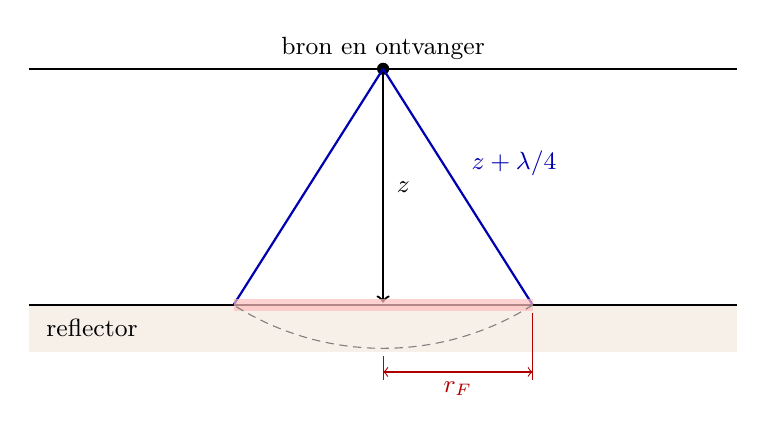
\begin{tikzpicture}[font=\small, x=1cm, y=1cm]
\fill[brown!12] (-4.5,-3.6) rectangle (4.5,-3.0);
\draw[thick] (-4.5,-3.0) -- (4.5,-3.0);
\node[anchor=north west] at (-4.4,-3.05) {reflector};
\draw[thick] (-4.5,0) -- (4.5,0);
\fill (0,0) circle (2.2pt) node[above] {bron en ontvanger};
\draw[->, thick] (0,0) -- (0,-2.97);
\node[anchor=west] at (0.05,-1.5) {$z$};
\draw[blue!70!black, thick] (0,0) -- (1.9,-3.0);
\draw[blue!70!black, thick] (0,0) -- (-1.9,-3.0);
\node[anchor=west, blue!70!black] at (1.0,-1.2) {$z + \lambda/4$};
\fill[red!25, opacity=0.7] (-1.9,-3.08) rectangle (1.9,-2.92);
\draw[red!70!black] (0,-3.65) -- (0,-3.95) (1.9,-3.1) -- (1.9,-3.95);
\draw[<->, red!70!black] (0,-3.85) -- (1.9,-3.85) node[midway, below] {$r_F$};
\draw[gray, densely dashed] (-57.6:3.55) arc (-57.6:-122.4:3.55);
\end{tikzpicture}

\par\smallskip{\small De eerste \omterm{def:b3:exploration-seismology:fresnel}{Fresnelzone} (schematisch): het deel van de
reflector waarvan de afstand tot een samenvallende bron en ontvanger de
loodrechte afstand $z$ met minder dan $\lambda/4$ overschrijdt (gestreepte boog: de bol met straal
$z + \lambda/4$), zodat het heen-en-terugextra pad minder dan een halve golflengte bedraagt
en de echo's in fase aankomen. De schaal van $\lambda$ is overdreven.}
\label{fig:b3:exploration-seismology:fresnel}
\end{omfigure}

\section{Gemeenschappelijk-middelpuntmeting en verwerking}

Een enkele echo is in de ruis te zwak om te zien. Reflectieonderzoeken registreren
daarom elk punt in de ondergrond vele malen, met verschillende bron-ontvangerparen,
en tellen de registraties op.

\begin{definition}[Gemeenschappelijk middelpunt, bedekkingsgraad]\label{def:b3:exploration-seismology:cmp}
Voor een bron op $x_s$ en een ontvanger op $x_r$ op één lijn is het middelpunt
$(x_s + x_r)/2$ en de offset $x = |x_r - x_s|$. Een \emph{gemeenschappelijk
middelpunt}\index{gemeenschappelijk middelpunt} (CMP) verzameling is de set sporen, van alle
schoten, die hetzelfde middelpunt delen; bij vlakke lagen reflecteren ze allemaal aan
hetzelfde punt in de ondergrond. De \emph{bedekkingsgraad (van seismische dekking)}\index{bedekkingsgraad (van seismische dekking)}
is het aantal sporen in een verzameling. Met $N$ kanalen op de ontvangerafstand $\Delta g$ en
een schot elke $\Delta s$ langs de lijn is de bedekkingsgraad
$N\Delta g/(2\Delta s)$.
\end{definition}

\begin{omfigure}
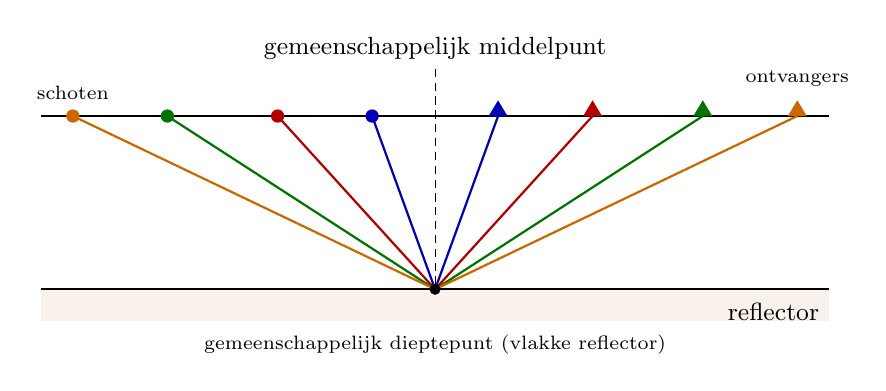
\begin{tikzpicture}[font=\small, x=1cm, y=1cm]
\draw[thick] (-5,0) -- (5,0);
\fill[brown!10] (-5,-2.6) rectangle (5,-2.2);
\draw[thick] (-5,-2.2) -- (5,-2.2);
\node[anchor=north east] at (5,-2.25) {reflector};
\foreach \off/\col in {0.8/blue!70!black, 2.0/red!70!black, 3.4/green!45!black, 4.6/orange!80!black} {
  \draw[\col, thick] (-\off,0) -- (0,-2.2) -- (\off,0);
  \fill[\col] (-\off,0) circle (2.4pt);
  \fill[\col] (\off-0.12,0) -- (\off+0.12,0) -- (\off,0.2) -- cycle;
}
\fill (0,-2.2) circle (2pt);
\draw[densely dashed] (0,0.6) -- (0,-2.2);
\node[anchor=south] at (0,0.6) {gemeenschappelijk middelpunt};
\node[anchor=north, align=center, font=\scriptsize] at (0,-2.65) {gemeenschappelijk dieptepunt (vlakke reflector)};
\node[anchor=south, font=\scriptsize] at (-4.6,0.08) {schoten};
\node[anchor=south, font=\scriptsize] at (4.6,0.25) {ontvangers};
\end{tikzpicture}

\par\smallskip{\small Geometrie van het \omterm{def:b3:exploration-seismology:cmp}{gemeenschappelijk middelpunt} (schematisch): vier bron--ontvangerparen
(bolletjes, driehoeken) met verschillende offsets delen hetzelfde middelpunt; boven een
vlakke reflector weerkaatsen ze allemaal op hetzelfde punt eronder. Hun sporen vormen een
verzameling met bedekkingsgraad vier.}
\label{fig:b3:exploration-seismology:cmp}
\end{omfigure}

\begin{theorem}[Normal moveout (NMO)]\label{thm:b3:exploration-seismology:nmo}
In een laag met snelheid $v$ boven een vlakke reflector op de verticale tweewegtijd
$t_0$ bereikt de bij offset $x$ geregistreerde reflectie op
\[
  t(x)^2 = t_0^2 + \frac{x^2}{v^2},
\]
een hyperbool in het $(x, t)$-vlak. De vertraging $\Delta t = t(x) - t_0$ is de
\emph{normal moveout}\index{normal moveout}; voor $x \ll vt_0$,
$\Delta t \approx x^2/(2v^2t_0)$.
\end{theorem}

\begin{proof}
De reflectieweg loopt van de bron naar het reflectiepunt onder het
middelpunt en weer omhoog naar de ontvanger: twee takken met lengte
$\sqrt{(vt_0/2)^2 + (x/2)^2}$. Dus $t = (2/v)\sqrt{(vt_0/2)^2 + (x/2)^2}$ en
$t^2 = t_0^2 + x^2/v^2$. Dan $t - t_0 = (t^2 - t_0^2)/(t + t_0) \approx
x^2/(2v^2t_0)$.
\end{proof}

Bij meerdere lagen is de reflectietijd niet langer exact hyperbolisch, maar
bij kleine offsets is ze dat vrijwel wel, met een snelheid die een gewogen gemiddelde is van de
lagen.

\begin{definition}[Stapelsnelheid, RMS-snelheid en intervalsnelheden]\label{def:b3:exploration-seismology:velocities}
De \emph{intervalsnelheid}\index{intervalsnelheid} $v_i$ van een laag is de
eigen snelheid; met $\Delta t_i = 2h_i/v_i$ de tweewegtijd erdoorheen, de
\emph{RMS-snelheid}\index{RMS-snelheid} tot aan de
onderkant van laag $n$ is
\[
  V_{\text{rms},n} = \left(\frac{\sum_{i\le n}v_i^2\,\Delta t_i}{\sum_{i\le n}\Delta t_i}\right)^{1/2}.
\]
De \emph{stapelsnelheid}\index{stapelsnelheid} van een reflectie is de
snelheid $V$ van de hyperbool $t^2 = t_0^2 + x^2/V^2$ die zijn tijden het best past in een
CMP-verzameling.
\end{definition}

\begin{proposition}[Stapelsnelheid bij kleine offsets]\label{prop:b3:exploration-seismology:rms}
Bij vlakke lagen geldt $t(x)^2 = t_0^2 + x^2/V_{\text{rms}}^2 + O(x^4)$: bij kleine
offsets is de \omterm{def:b3:exploration-seismology:velocities}{stapelsnelheid} gelijk aan de \omterm{def:b3:exploration-seismology:velocities}{RMS-snelheid}.
\end{proposition}

\begin{proof}
Voor de \omterm{def:b3:seismology-imaging:ray-parameter}{straalparameter} $p$ geldt $x = \sum_i 2h_i\tan\varphi_i$ en
$t = \sum_i 2h_i/(v_i\cos\varphi_i)$, met $\sin\varphi_i = pv_i$. Tot de tweede
orde in $p$ geldt $\tan\varphi_i \approx pv_i$ en $1/\cos\varphi_i \approx 1 +
p^2v_i^2/2$, dus $x \approx p\sum v_i^2\Delta t_i = pV_{\text{rms}}^2t_0$ en
$t \approx t_0 + \tfrac12p^2V_{\text{rms}}^2t_0$. Dan
$t^2 \approx t_0^2 + p^2V_{\text{rms}}^2t_0^2 = t_0^2 + x^2/V_{\text{rms}}^2$, waarbij
de verwaarloosde termen van orde $p^4$ zijn, dus van orde $x^4$.
\end{proof}

\begin{theorem}[Dix-vergelijking]\label{thm:b3:exploration-seismology:dix}
Als $V_{n-1}$ en $V_n$ de RMS-snelheden zijn tot de bovenkant en de onderkant van laag
$n$, op de tweewegtijden $t_{n-1}$ en $t_n$, wordt de \omterm{def:b3:exploration-seismology:velocities}{intervalsnelheid} van de
laag gegeven door de \emph{Dix-vergelijking}\index{Dix-vergelijking}
\[
  v_n^2 = \frac{V_n^2t_n - V_{n-1}^2t_{n-1}}{t_n - t_{n-1}} ,
\]
en de dikte is $h_n = v_n(t_n - t_{n-1})/2$.
\end{theorem}

\begin{proof}
Per definitie is $V_n^2t_n = \sum_{i\le n}v_i^2\Delta t_i$ en $V_{n-1}^2t_{n-1}
= \sum_{i\le n-1}v_i^2\Delta t_i$. Hun verschil is $v_n^2\Delta t_n$, met
$\Delta t_n = t_n - t_{n-1}$.
\end{proof}

Snelheidsanalyse doorzoekt elke verzameling naar de hyperbool die het best past bij de
energie: voor elke proefwaarde van $t_0$ en $V$ worden de sporen langs de kromme opgeteld, en
wordt een coherentiemaat (de semblance) in kaart gebracht; de analist kiest de maxima,
reflector voor reflector, om een snelheidsfunctie op te bouwen. De NMO-correctie
verschuift vervolgens elk monster van elk spoor van $t(x)$ naar $t_0$, waarmee de
reflecties vlak worden getrokken, en de sporen van elke verzameling worden opgeteld.

\begin{definition}[Stapeling (seismisch)]\label{def:b3:exploration-seismology:stack}
\emph{Stapeling (seismisch)}\index{stapeling (seismisch)} is de optelling, na de
NMO-correctie, van de sporen van een CMP-verzameling tot één spoor
geplaatst op het middelpunt. De gestapelde sporen, naast elkaar langs de lijn, vormen
de gestapelde sectie, een beeld van de reflectoren in tweewegtijd.
\end{definition}

\begin{proposition}[Winst van een stapeling]\label{prop:b3:exploration-seismology:sqrtN}
Als de $N$ sporen van een verzameling hetzelfde reflectiesignaal dragen en onafhankelijke
ruis met gelijke standaarddeviatie $\sigma$ hebben, dan draagt hun gemiddelde hetzelfde signaal
en ruis met standaarddeviatie $\sigma/\sqrt N$: stapeling verhoogt de
signaal-ruisverhouding met een factor $\sqrt N$.
\end{proposition}

\begin{proof}
De variantie van een som van $N$ onafhankelijke variabelen is de som van hun
varianties, $N\sigma^2$; gedeeld door $N^2$ heeft het gemiddelde de variantie
$\sigma^2/N$ (de standaarddeviatie van het gemiddelde, bekend uit de
wiskundeboeken).
\end{proof}

\begin{omfigure}
\begin{tikzpicture}
\begin{groupplot}[group style={group size=2 by 1, horizontal sep=0.5cm, y descriptions at=edge left},
  width=0.52\linewidth, height=0.56\linewidth, y dir=reverse, ymin=0.4, ymax=0.92,
  xmin=-150, xmax=2150, tick label style={font=\scriptsize}, title style={font=\small},
  xlabel={\scriptsize offset (\unit{m})}]
\nextgroupplot[title={(a) CMP-verzameling}, ylabel={tweewegtijd (\unit{s})}]
\addplot[black, very thin, unbounded coords=jump] table[x=x, y=t] {figdata/out/bachelor-3-cmp_nmo-gather-raw.dat};
\nextgroupplot[title={(b) na NMO-correctie}]
\addplot[black, very thin, unbounded coords=jump] table[x=x, y=t] {figdata/out/bachelor-3-cmp_nmo-gather-nmo.dat};
\end{groupplot}
\end{tikzpicture}

\par\smallskip{\small Een synthetische CMP-verzameling onder de synclinaleas van de
Varden-lijn (berekend met exacte straalvolging door de vlakgelaagde kolom; \omterm{def:b3:exploration-seismology:wavelet}{Ricker-wavelet} van 30
Hz; zonder ruis). (a) De vier reflecties (bovenkant van de schalie, bovenkant
en onderkant van de kalksteen, bovenkant van het basement) buigen met de offset
omlaag langs bijna-hyperbolen. (b) Na de NMO-correctie met de stapelsnelheden
gepast op de offsets tot \qty{600}{m}, liggen de reflecties tot ongeveer
\qty{1}{km} vlak; daarachter wijken de werkelijke tijden af van de hyperbool en
laat de correctie ze gebogen, en zijn de wavelets uitgerekt; bij de verwerking
worden de uitgerekte verre sporen van de ondiepe reflecties vóór de
stapeling gedempt.}
\label{fig:b3:exploration-seismology:gather}
\end{omfigure}

\begin{omfigure}
\begin{tikzpicture}
\begin{axis}[omrecord, width=0.72\linewidth, height=0.46\linewidth,
  xmin=0.4, xmax=0.78, ymin=2000, ymax=5000,
  xlabel={tweewegtijd $t_0$ (\unit{s})}, ylabel={snelheid (\unit{m.s^{-1}})},
  legend cell align=left, legend columns=2,
  legend style={font=\scriptsize, at={(0.5,-0.24)}, anchor=north}]
\addplot[gray, thick, const plot mark right] table[x=t0, y=vint] {figdata/out/bachelor-3-cmp_nmo-vel.dat};
\addlegendentry{intervalsnelheid van het model}
\addplot[gray, thick, forget plot] coordinates {(0.4,2500) (0.487847,2500)};
\addplot[blue!70!black, thick, mark=*, mark size=1.5pt] table[x=t0, y=vrms] {figdata/out/bachelor-3-cmp_nmo-vel.dat};
\addlegendentry{RMS-snelheid}
\addplot[red!70!black, only marks, mark=square*, mark size=1.6pt] table[x=t0, y=vstack] {figdata/out/bachelor-3-cmp_nmo-vel.dat};
\addlegendentry{stapelsnelheid (offsets tot \qty{600}{m})}
\addplot[green!45!black, only marks, mark=triangle*, mark size=2pt] table[x=t0, y=vdix] {figdata/out/bachelor-3-cmp_nmo-vel.dat};
\addlegendentry{Dix-intervalsnelheid}
\end{axis}
\end{tikzpicture}

\par\smallskip{\small Snelheden onder de synclinaleas (berekend). De \omterm{def:b3:exploration-seismology:velocities}{RMS-snelheid}, een
gewogen gemiddelde, verandert langzaam; de stapelsnelheden van de verzameling
liggen er dicht bij. Toegepast op deze snelheden herstelt de \omterm{thm:b3:exploration-seismology:dix}{Dix-vergelijking} de \omterm{def:b3:exploration-seismology:velocities}{intervalsnelheid}
van elke laag (de trapvormige lijn, getekend aan de onderkant van elke laag) tot
binnen enkele procenten, waarbij de fout groeit in de dunne, snelle kalksteen.}
\label{fig:b3:exploration-seismology:velocities}
\end{omfigure}

\begin{omfigure}
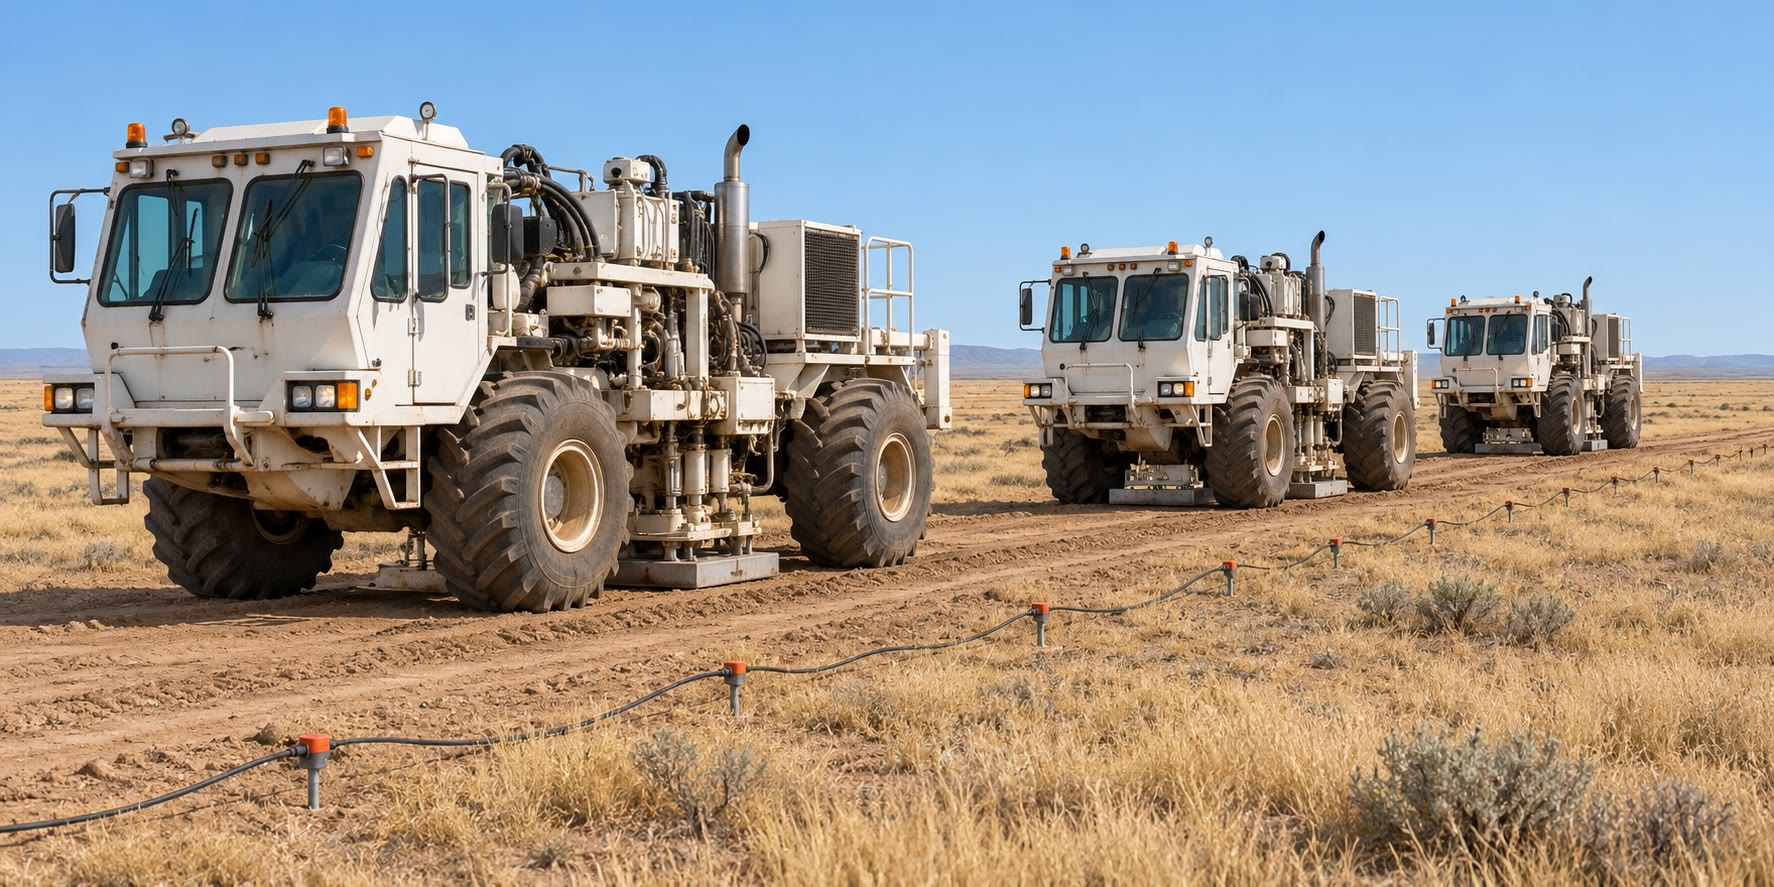
\includegraphics[width=0.62\linewidth]{images/book5/ai/b3-vibroseis.jpg}

\par\smallskip{\small Trillingswagens op een landmeetlijn: in plaats van een
explosie drukt elke wagen een zware plaat op de grond en laat die gedurende enkele
seconden trillen met een sweep van frequenties; de lange registraties worden
samengedrukt tot korte pulsen door ze te correleren met de sweep (Door AI gegenereerde illustratie.)}
\label{fig:b3:exploration-seismology:vibroseis}
\end{omfigure}

\section{Migratie}

Een gestapelde sectie toont elke reflectie onder het middelpunt waar ze werd
geregistreerd, op het tijdstip dat de echo nodig had om terug te keren. Voor een vlakke
reflector klopt dat. Voor een hellende reflector niet: de echo die op een oppervlaktepunt
wordt geregistreerd, komt van het punt van de reflector dat er het dichtst bij ligt;
dat ligt bergopwaarts, niet recht eronder. Punten zoals breukuiteinden, die energie naar alle
richtingen verstrooien, verschijnen als hyperbolen.

\begin{definition}[Seismische migratie]\label{def:b3:exploration-seismology:migration}
\emph{Seismische migratie}\index{seismische migratie} is de verwerkingsstap die
de reflecties van een seismische sectie verplaatst naar de posities van de reflectoren
die ze hebben veroorzaakt: zij herstelt de werkelijke hellingen en posities van
hellende reflectoren en herleidt de diffractiehyperbolen van puntverstrooiers tot hun
toppen. Uitgevoerd met een snelheidsmodel in tijd levert zij een tijdgemigreerde
sectie op; met een model in diepte een dieptebeeld.
\end{definition}

\begin{theorem}[Helling op een sectie bij nuloffset]\label{thm:b3:exploration-seismology:dip}
In een medium met snelheid $v$ verschijnt een vlakke reflector met helling $\theta$ in het
vlak van de sectie op de sectie bij nuloffset, uitgezet als de diepte $vt/2$
recht onder elk registratiepunt, als een lijn met schijnbare helling $\theta_a$
met
\[
  \tan\theta_a = \sin\theta .
\]
De reflectie die in het punt $x$ wordt geregistreerd, komt van het reflectorpunt op een
afstand $(vt/2)\sin\theta$ bergopwaarts van het punt recht onder $x$.
\end{theorem}

\begin{proof}
De straal bij nuloffset staat loodrecht op de reflector, zodat de in $x$ geregistreerde tijd is
$t = 2d(x)/v$, waarbij $d(x)$ de afstand van $x$ tot het vlak is. Die afstand
neemt toe met $\sin\theta$ per eenheid van $x$ in de richting van de helling, zodat de
uitgezette diepte $vt/2 = d(x)$ heeft de helling $\sin\theta$. De voet van de loodlijn vanuit $x$
op het vlak ligt op de horizontale afstand $d\sin\theta$ van $x$, aan de
bergopwaartse kant.
\end{proof}

Omdat $\tan\theta_a = \sin\theta < \tan\theta$, toont een ongemigreerde sectie altijd
hellingen die vlakker zijn dan de werkelijke, en kan zij helemaal geen hellingen steiler dan
\ang{45} tonen. Een puntverstrooier op diepte $z$ onder het punt $x_0$ geeft bij
$x$ de nultijd $t(x) = (2/v)\sqrt{z^2 + (x - x_0)^2}$: een hyperbool met
haar top boven het punt, de diffractie. Migratie in de eenvoudigste vorm,
de diffractiestapeling, somt elke sectie langs de diffractiehyperbool van
elke mogelijke verstrooier op en plaatst de som in de top: reflectoren, die
continue lijnen van verstrooiers zijn, komen op hun werkelijke plaats tevoorschijn, en
de diffracties worden samengetrokken.

\begin{omfigure}
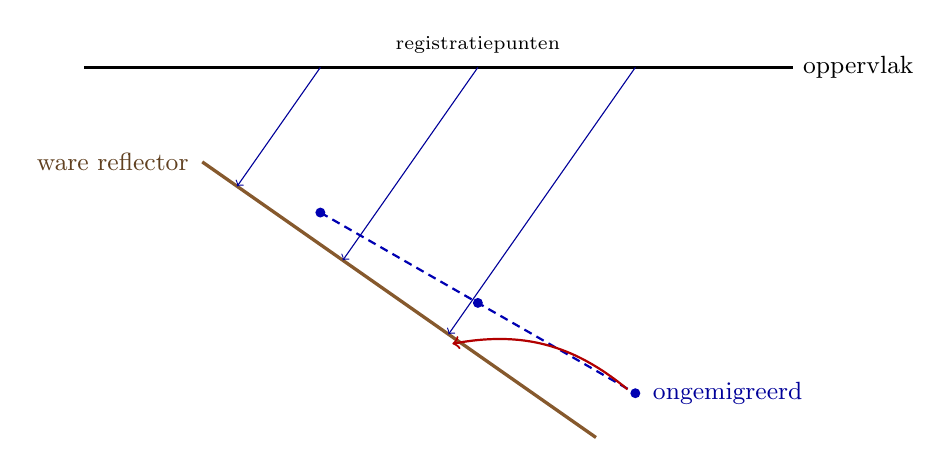
\begin{tikzpicture}[font=\small, x=1cm, y=1cm]
\draw[thick] (-0.5,0) -- (8.5,0) node[right] {oppervlak};
% true reflector, dip 35 deg, rising to the left
\draw[very thick, brown!70!black] (1.0,-1.2) -- (6.0,-4.70);
\node[brown!50!black, anchor=east] at (0.95,-1.2) {ware reflector};
% zero-offset normal rays from x = 2, 4, 6
\foreach \x in {2.5, 4.5, 6.5} {
  % distance from (x,0) to the line through (1,-1.2) dir (cos35,-sin35): normal n=(sin35,cos35)
  \pgfmathsetmacro{\dd}{abs(0.5736*(\x-1.0) + 0.8192*(0+1.2))}
  \draw[blue!60!black, ->] (\x,0) -- ++({-0.5736*\dd},{-0.8192*\dd});
  \fill[blue!70!black] (\x,{-\dd}) circle (1.8pt);
}
% apparent reflector through the plotted points
\pgfmathsetmacro{\da}{abs(0.5736*1.5 + 0.8192*1.2)}
\pgfmathsetmacro{\db}{abs(0.5736*5.5 + 0.8192*1.2)}
\draw[blue!70!black, thick, densely dashed] (2.5,{-\da}) -- (6.5,{-\db});
\node[blue!60!black, anchor=west] at (6.6,{-\db}) {ongemigreerd};
\node[anchor=south, font=\scriptsize] at (4.5,0.05) {registratiepunten};
\draw[->, red!70!black, thick] (6.4,{-\db+0.05}) to[bend right=25] ({6.5-0.5736*\db+0.05},{-0.8192*\db-0.12});
\end{tikzpicture}

\par\smallskip{\small Migratie van een hellende reflector (schematisch, ware helling
\ang{35}). De zero-offsetstraal bij elk registratiepunt staat loodrecht op de
reflector, dus de echo komt van bergopwaarts; loodrecht onder het punt uitgezet,
op de diepte $vt/2$, lijkt de reflectie flauwer (gestreept: $\tan\theta_a =
\sin\theta$, hier \ang{29.8}), en is bergafwaarts verschoven. Migratie (rode pijl) brengt haar terug.}
\label{fig:b3:exploration-seismology:migration}
\end{omfigure}

\section{Seismische stratigrafie}

Een gemigreerde sectie is een beeld van de gelaagdheid, en ze kan worden gelezen als
stratigrafie: de reflecties volgen de lagvlakken, die
tijdlijnen zijn, dus hun geometrie legt vast hoe het bekken is gevuld.

\begin{definition}[Seismische stratigrafie, seismische facies]\label{def:b3:exploration-seismology:seismic-stratigraphy}
\emph{Seismische stratigrafie}\index{seismische stratigrafie} is de interpretatie
van de stratigrafie en de afzettingsgeschiedenis van een bekken aan de hand van de geometrie
van zijn seismische reflecties. Een \emph{seismische facies}\index{seismische facies} is een
driedimensionale eenheid van reflecties waarvan het karakter (continuïteit, amplitude,
frequentie, interne geometrie: parallel, divergent, sigmoïdaal, chaotisch, bolvormig)
wijkt af van dat van de buureenheden en wordt geïnterpreteerd als een
afzettingsmilieu.
\end{definition}

\begin{definition}[Reflectiebeëindigingen]\label{def:b3:exploration-seismology:terminations}
Een \emph{reflectiebeëindiging}\index{reflectiebeëindiging} is het einde van een
reflectie tegen een andere. \emph{Onlap}\index{onlap}: een aanvankelijk horizontale
reflectie eindigt tegen een oppervlak dat steiler stijgt, de jongere lagen
liggen aan tegen een oudere helling. \emph{Downlap}\index{downlap}: een hellende
reflectie eindigt bergafwaarts tegen een flauwer oppervlak, omdat de voeten van prograderende
lagen op de bodem van een bekken rusten. \emph{Toplap}\index{toplap}: hellende
reflecties eindigen bergopwaarts tegen een bovenliggend oppervlak, met weinig erosie, omdat
de toppen van prograderende lagen het niveau van de zee raken. \emph{Erosieve
afknotting}\index{erosieve afknotting}: reflecties eindigen bergopwaarts tegen een
bovenliggend oppervlak dat ze afsnijdt, een discordantie.
\end{definition}

\begin{omfigure}
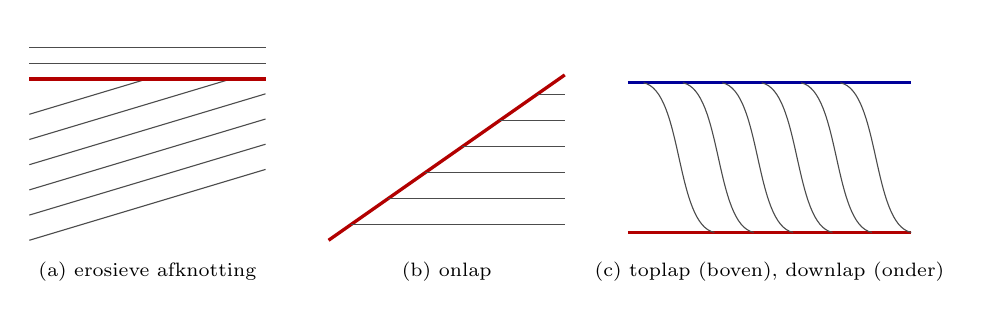
\begin{tikzpicture}[font=\scriptsize, x=1cm, y=1cm]
% erosional truncation: tilted beds cut by an unconformity
\begin{scope}
\foreach \k in {0,...,5} {\draw[gray!60!black] (0,{-2.3+0.32*\k}) -- (3.0,{-1.4+0.32*\k-0.25*0});}
\fill[white] (0,-0.25) -- (3.2,-0.25) -- (3.2,0.4) -- (0,0.4) -- cycle;
\draw[very thick, red!70!black] (0,-0.25) -- (3.0,-0.25);
\foreach \k in {0,1} {\draw[gray!60!black] (0,{-0.05+0.2*\k}) -- (3.0,{-0.05+0.2*\k});}
\node[anchor=north] at (1.5,-2.45) {(a) erosieve afknotting};
\end{scope}
% onlap
\begin{scope}[xshift=3.8cm]
\draw[very thick, red!70!black] (0,-2.3) -- (3.0,-0.2);
\foreach \k in {0,...,5} {\pgfmathsetmacro{\y}{-2.1+0.33*\k} \pgfmathsetmacro{\xe}{(\y+2.3)/0.7} \draw[gray!60!black] (\xe,\y) -- (3.0,\y);}
\node[anchor=north] at (1.5,-2.45) {(b) onlap};
\end{scope}
% downlap and toplap: clinoforms
\begin{scope}[xshift=7.6cm]
\draw[very thick, red!70!black] (0,-2.2) -- (3.6,-2.2);
\draw[very thick, blue!60!black] (0,-0.3) -- (3.6,-0.3);
\foreach \k in {0,...,5} {\draw[gray!60!black] ({0.2+0.5*\k},-0.3) .. controls ({0.7+0.5*\k},-0.4) and ({0.6+0.5*\k},-2.1) .. ({1.1+0.5*\k},-2.2);}
\node[anchor=north] at (1.8,-2.45) {(c) toplap (boven), downlap (onder)};
\end{scope}
\end{tikzpicture}

\par\smallskip{\small \omterm{def:b3:exploration-seismology:terminations}{Reflectiebeëindigingen} (schematische secties, grijze
reflecties, beëindigende vlakken in kleur). (a) Gekantelde reflecties die door een
discordantie zijn afgesneden. (b) Vlakke reflecties die eindigen tegen een oudere helling. (c) Hellende
lagen van een prograderende wig die bergopwaarts eindigen tegen het oppervlak erboven (\omterm{def:b3:exploration-seismology:terminations}{toplap}) en
bergafwaarts op de bekkenbodem (\omterm{def:b3:exploration-seismology:terminations}{downlap}).}
\label{fig:b3:exploration-seismology:terminations}
\end{omfigure}

De beëindigingen markeren de vlakken die reeksen genetisch verwante
lagen begrenzen. Ze over een bekken in kaart brengen en ze relateren aan het stijgen en dalen van
het relatieve zeeniveau, is sequentiestratigrafie, het onderwerp van
\cref{ch:b3:sequence-stratigraphy}. Een seismische sectie van een passieve rand toont
meestal wiggen van naar zee prograderende reflecties die downlappen op de
diepe bodem, afgesloten door \omterm{def:b3:exploration-seismology:terminations}{toplap}, en landwaarts begraven onder onlapende lagen die
werden afgezet toen de zee weer steeg.

\begin{inthefield}[Een mariene streamersurvey en een landploeg]
\begin{minipage}[t]{0.55\linewidth}\vspace{0pt}
Bij een mariene survey stopt het schip nooit: het vaart lijn na lijn met enkele
knopen, de luchtkanonarrays vuren op vaste intervallen, en de streamers worden op een
constante diepte gehouden door kleine stuurbare vleugels en gelokaliseerd met
akoestische en satellietpositionering. Waarnemers op de brug houden de zee rond de array in de gaten, en de
survey werkt onder regels die de maatregelen vastleggen om zeezoogdieren te beschermen, de
wacht die wordt gehouden en wat er wordt gerapporteerd.
% ledger: noaa5:itr-gom
Op land legt de ploeg kabels of draadloze registratie-eenheden langs de lijnen aan;
vibratorwagens rijden in konvooi van het ene bronpunt naar het volgende, en een
registratiewagen controleert elk kanaal voor elke veegbeweging. Terug in het
verwerkingscentrum worden de registraties gesorteerd in verzamelingen met een \omterm{def:b3:exploration-seismology:cmp}{gemeenschappelijk
middelpunt}, de snelheden gekozen, de data gestapeld en gemigreerd, en de sectie aan de
interpreteurs overgedragen.
\end{minipage}\hfill
\begin{minipage}[t]{0.42\linewidth}\vspace{0pt}
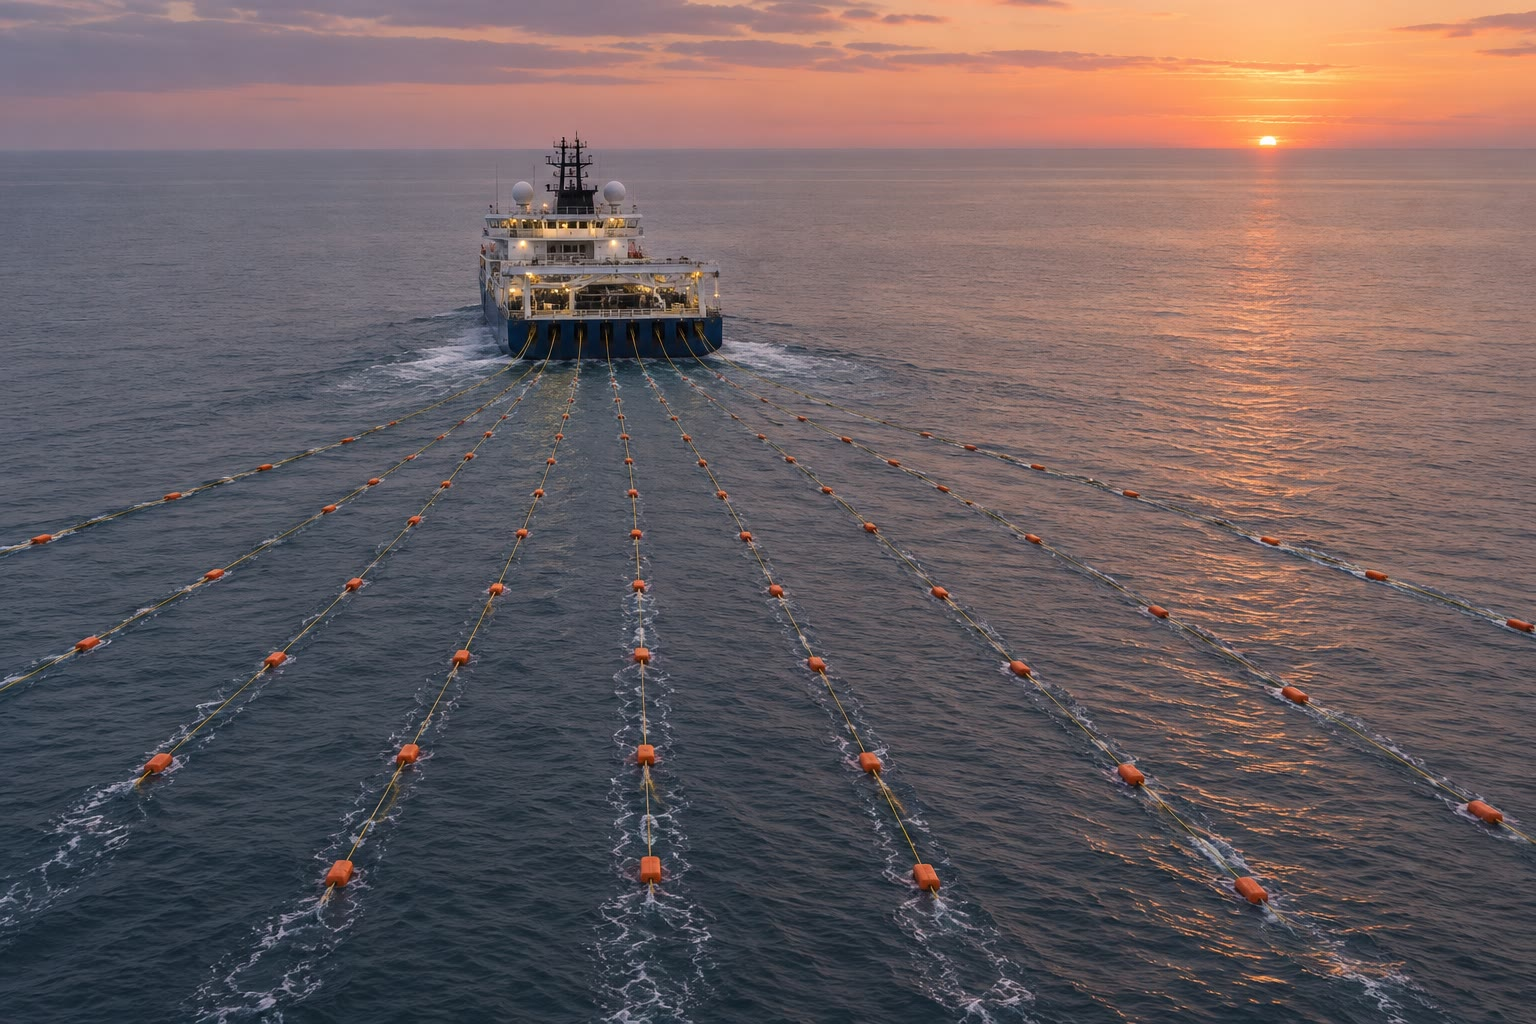
\includegraphics[width=\linewidth]{images/book5/ai/b3-streamer-vessel.jpg}

{\scriptsize Een seismisch onderzoeksschip dat zijn streamers bij schemering achter zich aan sleept
(Door AI gegenereerde illustratie.)}
\end{minipage}
\end{inthefield}

\section{Oefeningen}

\begin{exercise}[$\star$]\label{exo:b3:exploration-seismology:1}
Krijt ($v = \qty{2500}{m.s^{-1}}$, $\rho = \qty{2.00}{g.cm^{-3}}$) ligt op schalie
(\qty{2300}{m.s^{-1}}, \qty{2.30}{g.cm^{-3}}), dat op kalksteen ligt
(\qty{4500}{m.s^{-1}}, \qty{2.60}{g.cm^{-3}}). Bereken de drie impedanties en
de reflectiecoëfficiënten van de twee grensvlakken. Welk deel van de invallende
energie reflecteert de bovenkant van de kalksteen?
% ledger: mavko:velocities
\end{exercise}

\begin{exercise}[$\star$]\label{exo:b3:exploration-seismology:2}
Een vlakke reflector ligt \qty{800}{m} onder een laag met \qty{2000}{m.s^{-1}}.
Bereken $t_0$, de reflectietijd bij een offset van \qty{1000}{m}, en de \omterm{thm:b3:exploration-seismology:nmo}{normal
moveout} daar. Vergelijk met de benadering $x^2/(2v^2t_0)$.
\end{exercise}

\begin{exercise}[$\star$]\label{exo:b3:exploration-seismology:3}
Een streamer heeft 240 kanalen op \qty{12.5}{m} van elkaar, en het schip schiet elke
\qty{25}{m}. Bereken het CMP-interval en de bedekkingsgraad. Welk schotinterval zou
een bedekkingsgraad van 120 geven?
\end{exercise}

\begin{exercise}[$\star$]\label{exo:b3:exploration-seismology:4}
Bereken bij een dominante frequentie van \qty{30}{Hz} de golflengte en de
kwartgolflengte in zandsteen van \qty{3000}{m.s^{-1}} en in kalksteen van
\qty{4500}{m.s^{-1}}. Bereken de straal van de eerste \omterm{def:b3:exploration-seismology:fresnel}{Fresnelzone} van een
reflector op \qty{1000}{m} diepte onder gesteenten met een gemiddelde snelheid van \qty{2800}{m.s^{-1}}.
\end{exercise}

\begin{exercise}[$\star\star$]\label{exo:b3:exploration-seismology:5}
Twee reflecties hebben $t_0 = \qty{0.500}{s}$ met een \omterm{def:b3:exploration-seismology:velocities}{RMS-snelheid} van
\qty{2400}{m.s^{-1}}, en $t_0 = \qty{0.700}{s}$ met \qty{2800}{m.s^{-1}}.
Bereken de \omterm{def:b3:exploration-seismology:velocities}{intervalsnelheid} en de dikte van de laag ertussen.
\end{exercise}

\begin{exercise}[$\star\star$]\label{exo:b3:exploration-seismology:6}
Een vlakke reflector heeft een helling van $\varphi$ in het vlak van een CMP-lijn, in een laag met
snelheid $v$. (a) Toon aan dat $t(x)^2 = t_0^2 + x^2\cos^2\varphi/v^2$, waarbij $t_0$
de nul-offsettijd in het middelpunt is. (Hint: gebruik het spiegelbeeld van het middelpunt in
de reflector.) (b) Leid de \omterm{def:b3:exploration-seismology:velocities}{stapelsnelheid} af en bereken die voor
$v = \qty{2000}{m.s^{-1}}$ en $\varphi = \ang{12}$.
\end{exercise}

\begin{exercise}[$\star\star$]\label{exo:b3:exploration-seismology:7}
Een verzameling met bedekkingsgraad 60 heeft onafhankelijke ruis van gelijke variantie op elk spoor. Met
welke factor verhoogt stapeling de signaal-ruisverhouding? Met welke factor moet
de bedekkingsgraad worden verhoogd om de verhouding opnieuw te verdubbelen?
\end{exercise}

\begin{exercise}[$\star\star$]\label{exo:b3:exploration-seismology:8}
Op een nul-offsettijdsectie, in gesteente van \qty{3000}{m.s^{-1}}, stijgt een reflectie
met \qty{0.40}{s} dubbele looptijd per kilometer langs de lijn. Reken deze
helling om naar een schijnbare helling en bereken de werkelijke helling van de reflector.
\end{exercise}

\begin{exercise}[$\star\star$]\label{exo:b3:exploration-seismology:9}
Convolueer de \omterm{def:b3:exploration-seismology:synthetic}{reflectiviteitsreeks} $r = (0, 0.3, 0, -0.2, 0)$ met de
wavelet $w = (-0.5, 1, -0.5)$ van drie monsters, monster voor monster. Waar liggen de twee
reflecties, en overlappen zij elkaar?
\end{exercise}

\begin{exercise}[$\star\star\star$]\label{exo:b3:exploration-seismology:10}
Een omgekeerd refractieprofiel over een laag met \qty{1800}{m.s^{-1}} geeft een
schijnbare snelheid omlaag langs de helling van \qty{2900}{m.s^{-1}} en een tegen de helling in van
\qty{4400}{m.s^{-1}}. Bereken de kritische hoek, de helling en de
snelheid van de refractor. Vergelijk die met het harmonisch gemiddelde van de twee
schijnbare snelheden.
\end{exercise}

\begin{exercise}[$\star\star\star$]\label{exo:b3:exploration-seismology:11}
In \cref{prop:b3:exploration-seismology:tuning} heeft een laag
reflectiecoëfficiënten $+R$ en $-R$. (a) Toon aan dat voor $\Delta t \ll T$ het samengestelde
signaal ongeveer $R\,\Delta t\,w'(t)$ is, de tijdsafgeleide van de wavelet
geschaald met de tweewegdikte van de laag. (b) Leg uit waarom een dunne laag toch
gedetecteerd kan worden, al is ze niet opgelost, en hoe de dikte uit de amplitude
geschat kan worden. (c) Twee lagen van hetzelfde gesteente, 5 en \qty{10}{m} dik, worden
afgebeeld met dezelfde wavelet: wat is de verhouding van hun amplitudes?
\end{exercise}

\begin{exercise}[$\star\star\star$]\label{exo:b3:exploration-seismology:12}
Een puntverstrooier ligt \qty{600}{m} onder de lijn, in gesteente van
\qty{3000}{m.s^{-1}}. (a) Schrijf de nul-offsettijd van zijn diffractie uit als functie van
de horizontale afstand $x$ tot het punt erboven, en bereken die bij $x = 0$
en \qty{300}{m}. (b) Toon aan dat de diffractie een hyperbool van de NMO-vorm is,
met snelheid $v/2$, en leg uit waarom een diffractie altijd sterker gekromd is dan een
reflectie met dezelfde toptijd. (c) Wat doet migratie ermee?
\end{exercise}

\section{Probleem: Een seismische lijn over de Varden Hills}

\begin{problem}[{Weekendprobleem --- refractie, snelheidsanalyse, dieptomzetting
en migratie langs doorsnede A--B van de Varden Hills}]
\label{pb:b3:exploration-seismology:1}
% values: calc/ch02.py, from figdata seismic_model.py, refraction_dip.py, cmp_nmo.py
Een seismische lijn wordt geschoten langs doorsnede A--B van de Varden Hills, het gebied van
de geologische kaarten uit de eerdere delen. De afstanden $s$ worden gemeten vanaf
A langs de lijn. De bedekking bestaat van boven af uit krijt, schalie (\qty{100}{m}),
kalksteen (\qty{180}{m}) en zandsteen (\qty{120}{m}), die discordant op een
schistfundament rust; de reeks is geplooid tot een antiklinaal en een synklinaal en doorsneden door een
afschuiving.

\medskip
\noindent\textbf{Deel I --- Een refractiespreiding op de westelijke flank.} Er is een spreiding van
\qty{1200}{m} aangelegd tussen de schotpunten W ($s = \qty{300}{m}$) en O
($s = \qty{1500}{m}$), op terrein dat als vlak wordt beschouwd. Het krijt en de schalie boven de
kalksteen worden behandeld als één laag met $v_1 = \qty{2.40}{km.s^{-1}}$. De
kopgolftijden die van de registraties worden afgelezen zijn, van W naar O, \qty{425.2}{ms} bij
\qty{800}{m} en \qty{486.1}{ms} bij \qty{1200}{m}; van O naar W,
\qty{372.4}{ms} bij \qty{800}{m} en \qty{486.1}{ms} bij \qty{1200}{m}.
\begin{enumerate}
  \item Bereken de twee schijnbare snelheden. Welk schotpunt ligt tegen de helling in?
  \item Bereken de kritische hoek en de helling van de refractor.
  \item Bereken de snelheid van de refractor. Welk gesteente is het?
  \item Bereken de intercepttijden en de loodrechte diepten van de
        refractor onder W en onder O.
  \item Reken ze om naar verticale diepten en controleer de helling aan de hand van de twee diepten.
  \item De schalie onder het krijt is trager dan het krijt. Wat maakt het
        \omterm{def:b3:exploration-seismology:surveys}{seismisch refractieonderzoek} ervan, en hoe vertekent dat de diepten?
\end{enumerate}

\noindent\textbf{Deel II --- Snelheidsanalyse bij CMP S.} Verder naar het oosten ligt CMP S
op de as van de syncline, in het neergezakte blok van de breuk, waar
de lagen als horizontaal worden beschouwd. Vier reflecties worden gekozen bij nulafstand en bij
\qty{600}{m}:
\begin{center}
\small
\begin{tabular}{lcccc}
\hline
reflectie & 1 & 2 & 3 & 4 \\
$t_0$ (\unit{s}) & 0.4878 & 0.5748 & 0.6548 & 0.7348 \\
$t(\qty{600}{m})$ (\unit{s}) & 0.5437 & 0.6240 & 0.6887 & 0.7648 \\
\hline
\end{tabular}
\end{center}
\begin{enumerate}[resume]
  \item Bereken de NMO-snelheid $V = x/\sqrt{t^2 - t_0^2}$ van reflecties 1
        en 2. Waarom is de tweede kleiner dan de eerste?
  \item Bereken die voor reflecties 3 en 4.
  \item Neem deze als RMS-snelheden en bereken met de
        \omterm{thm:b3:exploration-seismology:dix}{Dix-vergelijking} de \omterm{def:b3:exploration-seismology:velocities}{intervalsnelheid} van elke laag.
  \item Identificeer de lagen aan de hand van hun snelheden en noem de vier reflecterende
        grensvlakken.
  \item Reflectie 1 is de zwakste op de registraties. Waarom?
  \item Waarom zijn de snelheden alleen gemeten op afstanden tot \qty{600}{m},
        terwijl de spreiding \qty{2}{km} bereikt?
\end{enumerate}

\noindent\textbf{Deel III --- Diepteconversie en resolutie.}
\begin{enumerate}[resume]
  \item Bereken de tweewegtijd in elke laag en de dikte ervan.
  \item Bereken de diepte van elk reflecterend grensvlak onder het maaiveld. Vergelijk
        de diktes van de schalie, kalksteen en zandsteen met de
        hierboven gegeven waarden.
  \item Bereken de gemiddelde snelheid van het maaiveld tot aan het fundament en verklaar
        waarom de NMO-snelheid van reflectie 4 de diepte zou overschatten als die in plaats daarvan
        zou worden gebruikt.
  \item De \omterm{def:b3:exploration-seismology:wavelet}{seismische wavelet} van het onderzoek heeft zijn piek bij \qty{30}{Hz}. Bereken de golflengte in
        de schalie en de \omterm{def:b3:exploration-seismology:resolution}{tuningdikte}, zowel met de kwartgolflengteregel als met $b = v/(5.2f)$
        voor een \omterm{def:b3:exploration-seismology:wavelet}{Ricker-wavelet}. Is de schalie opgelost? Bij welke frequentie zou de schalie
        volgens de kwartgolflengteregel afgestemd zijn?
  \item Bereken de straal van de eerste \omterm{def:b3:exploration-seismology:fresnel}{Fresnelzone} op het fundament, met $\lambda$
        uit de NMO-snelheid van reflectie 4.
\end{enumerate}

\noindent\textbf{Deel IV --- Migratie en de breuk.}
\begin{enumerate}[resume]
  \item Nabij de breuk levert de afsnijding van de kalksteen een diffractie op waarvan de top
        op \qty{0.550}{s} ligt; \qty{200}{m} van de top langs de lijn ligt hij op
        \qty{0.5732}{s}. Geef de diffractietijd bij nulafstand en leid de
        gemiddelde snelheid boven de afsnijding af.
  \item Bereken de diepte van de afsnijding onder het maaiveld.
  \item Op de oostelijke flank stijgt de reflectie van de bovenkant van de kalksteen in de gestapelde
        sectie richting de antiklinaal met \qty{0.167}{s} heen-en-weertijd per
        kilometer, onder gesteenten met een gemiddelde snelheid van \qty{2.48}{km.s^{-1}}.
        Bereken de schijnbare helling en de werkelijke helling.
  \item Een reflectie op die flank wordt geregistreerd bij $t = \qty{0.655}{s}$. Hoe ver en in welke
        richting verplaatst migratie haar?
  \item Over de breuk springt de reflectie van de bovenkant van het fundament met \qty{0.160}{s};
        het neergezakte blok draagt de extra dikte in krijt. Bereken de
        verticale verplaatsing.
  \item Geef de diepte van de discordantie op het fundament onder CMP S, op basis van de
        intervalsnelheden uit deel II.
\end{enumerate}
\end{problem}
